\section{Implementation und Tests}
\subsection{Django Architektur}
Bei der Implementation der Anwendung befolgte man die vom Django Framework vorgegebene Architektur. Für die einzelnen Apps entschied man sich jedoch dafür, diese in einem separaten ''apps'' Verzeichnis zu speichern, um das Home-Verzeichnis übersichtlicher zu halten.\\

Django ist nach dem \gls{mtv} Pattern aufgebaut, was eine leichte Abänderung des \gls{mvc} Pattern ist. Beim \gls{mvc} Pattern dient das Model als Vermittler zwischen dem Website Interface und der Datenbank. Die View ist das eigentliche User Interface und enthält zum Beispiel das HTML oder CSS der Website. Der Controller ist die Hauptkomponente dieses Patterns und mappt anhand der vom Benutzer gestellten Anfrage das entrechende Model mit der entsprechenden View \footcite{django_mvc}. \\

<<<<<<< HEAD
Django basiert aber auf dem \gls{mtv} Pattern. Es kann etwas verwirrend sein, denn die einzelnen Rollen in \gls{mtv} wurden umbenannt. Der Controller wurde in View umbenannt und die View ist nun eigentlich die Templating-Engine\footcite{django_architektur}. Wird im Browser eine \gls{url} aufgerufen, entscheidet Django anhand der \gls{url} Patterns, an welche View die Anfrage gesendet wird. Diese View generiert dann schlussendlich die Webseite mit Hilfe des Templates. \\
=======
Django jedoch basiert auf dem \gls{mtv} Pattern. Es kann ein wenig verwirrend sein, denn die einzelnen Rollen im \gls{mtv} Pattern haben eine andere Bezeichnung als die im \gls{mvc} Pattern. Der Controller zum Beispiel wird als View bezeichnet und ist nun eigentlich die Templating-Engine\footcite{django_architektur}. Wird im Browser eine \gls{url} aufgerufen, entscheidet Django anhand des \gls{url} Patterns, an welche View die Anfrage gesendet wird. Diese View generiert dann schlussendlich die Webseite mit Hilfe des Templates. \\
>>>>>>> master

%Das Model enthält immer noch die logische Datenstruktur. Die View hat Zugriff auf das Model und kann so Daten speichern, updaten oder löschen. Erhält die View Daten vom Model, kann diese mit dem Template dargestellt werden. Das Template dient lediglich zur Darstellung der einzelnen Webseiten\footcite{django_mtv}.

\begin{figure}[H]
	\begin{center}	
		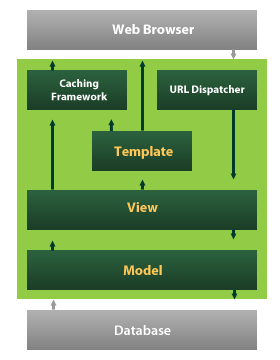
\includegraphics[width=0.5\textwidth, keepaspectratio]{images/django_mtv.png}
		\caption{Django Architektur Diagramm\footcite{django_architektur_image}}
			\label{django_architecture}
	\end{center}
\end{figure}

\subsubsection*{Model}
In den Models wird das Datenbankmodel mit den benötigten Attributen definiert\footcite{django_models}. Django stellt auch gleich einen \gls{orm} bereit, mit welchem die Tabellen in der Datenbank erstellt werden können. Dies bietet gleich meherere Vorteile. Zum einen nimmt der \gls{orm} viel Arbeit ab, da man keine eigenen Queries schreiben muss. Zum anderen ist er sehr hilfreich, wenn man Migrationen an der Datenstruktur durchführen möchte. Der \gls{orm} erkennt, was an der Datenbank geändert wurde und wie die Daten migriert werden muss\footcite{django_manage}. Als Entwickler können so auch ohne ausgeprägte Datenbank Kenntnisse Migrationen durchgeführt werden.

\subsubsection*{Templates}
Mit Templates können dynamische HTML Seiten generiert werden. Die Templates bestehen aus dem statischen HTML Code, welcher mit dynamischen Inhalten ergänzt werden kann.  Dazu verwendet Django die \gls{dtl}\footcite{django_templates}.

\subsubsection*{Views}
Eine View ist nichts anderes als eine Python Funktion, welche einen Request entgegen nimmt und eine Response zurück schicken. Die Response kann alles mögliche enthalten, von einfachem \gls{html} über 404 Fehlerseiten bis hin zu Redirects. Die View an sich enthält die Logik, welche nötig ist, um den Request entgegennehmen zu können und eine Response zu senden\footcite{django_views}.

\subsubsection*{Middlewares}
Hinzu kommen jedoch noch die Django Middlewares, welche Requests und Responses anpassen können. Jede dieser Middlewares ist für bestimmte Funktionen verantwortlich. Die ''AuthenticationMiddleware'' wird zum Beispiel verwendet, um die Benutzer einer Session zuordnen zu können. Es werden auch mehrere Security Middlewares angeboten, welche praktisch ''out-of-the-box'' verwendet werden können. Diese können die Sicherheit der Webseite, zum Beispiel die Integration von \gls{hsts} oder \gls{xss} Schutz, erhöhen\footcite{django_middlewares}.\\


%TODO vielleicht
%\subsection{Apps}
%Bei Django werden unabhängige Funktionalitäten in unterschiedliche Apps aufgeteilt. Eine App in Django ist eigentlich nichts anderes als ein Python Package, welches eine Reihe von Features zur Verfügung stellt\footcite{django:apps}. Das Ziel dabei ist es, den Code auf die verschiedenen Apps aufzuteilen, so dass diese unabhängig voneinander wiederverwendet werden können.  \\
%In der Tabelle \ref{table:django_apps} sind die einzelnen Apps aufgelistet, welche für Aufgaben-Coaching erstellt wurden.
%
%\begin{table}[h]
%	\centering
%	\begin{tabu} to 0.9\textwidth {l X}
%	\toprule
%	App & Beschreibung \\ 
%	\midrule	
%	user & In der Users App befindet sich die gesamte Logik zum erstellen und verwalten der User. \\
%	\midrule
%		school\_admin & Die school\_admin App ist für die Erstellung von Klassen sowie der Zuweisung von Schülern und Lehrern in Klassen zuständig. \\
%	\midrule
%	school\_teacher & In dieser App können Lehrer die Fächer für ihre Klasse freischalten und Aufgaben dem Wochenplan hinzufügen. \\
%	\midrule
%		exercise & Die exercise App stellt um Aufgaben zu erstellen zur Verfügung. Zudem können gelöste Aufgaben von einem Lehrer bewertet werden. \\
%	\midrule 
%	study\_content & Diese App beinhaltet die Logik zum bereitstellen von Lerninhalten \\
%	\midrule	
%	forum & In der forum App wird die komplette Logik für das Forum implementiert. \\
%	\bottomrule
%	\end{tabu}
%	\captionof{table}{Apps Beschreibung}
%	\label{table:django_apps}
%\end{table}


\subsection{Testing}
Es gibt mehrere Arten von Tests, welche durchgeführt wurden, um die Qulität dieser Arbeit zu gewährleisten.

\subsubsection{Unit Tests}
Anhand der Unittests werden die erstellten Models getestet. Mit diesen Tests wird sichergestellt, dass die Models korrekt funktionieren. Es kann zum Beispiel getestet werden, ob die Objekte als String abgespeichert werden oder ob duplizierte Objekte abgelegt werden können. Wenn in der Datenbank bereits ein Subject mit dem Titel ''Mathematik'' existiert, darf kein weiteres Subject mit dem selben Namen erstellt werden können.


\subsubsection{Integration Tests}
Mit Integration Tests kann getestet werden, ob die Applikation korrekt auf eingehende Requests reagiert. Diese Anwendung wird von mehreren Benutzern mit unterschiedlichen Rechten verwendet. Beim Erstellen der Tests wurde besonders viel Wert darauf gelegt, dass geprüft wird, dass jeder Benutzer nur Zugriff auf die erlaubten Webseiten hat. Aus Erfahrung weiss man, dass Schüler sehr experimentierfreudig sind und sicherlich versuchen werden, die \gls{url} des Browsers anzupassen. Es darf jedoch nicht vorkommen, dass ein Schüler Zugriff auf Statistiken hat oder die Punktezahl von Aufgaben anpassen kann.


\subsubsection{Manuelle Tests}
Manuelle Tests wurden da eingesetzt, wo es sehr schwierig und Zeitaufwändig gewesen wäre, Tests zu schreiben. Vor jedem Merge in den Master wurde geprüft, ob diese Funktionen noch funktionieren. Ein Beispiel für den Fall von manuellen Tests ist zum Beispiel, ob das Filtering und Pagination noch funktioniert. Zu Beginn hatte man da das Problem, dass das Filtern zwar funktionierte, aber das Pagination basierte auf dem gesamten Queryset. Die Anzahl der Seiten änderte sich also nicht, auch wenn der Filter kein einziges Element gefunden hat. Ein weiterer Fall für manuelle Tests sind die Drag\&Drop Seiten. Bei diesen wurde geprüft, ob man das Item einem Feld zuweisen kann und ob es anschliessend richtig in der Datenbank gespeichert wird. \\


\subsubsection{Usability Tests}
Nachdem man die Mockups erstellt hat, konnten damit die Usability Tests durchgeführt werden. Ziel dieser Tests ist es, zu prüfen, ob Benutzer das Design der Webseite verstehen und wissen, wo man was machen kann. \\

%TODO balsamiq i de mockups beschriibe, ned bim teste
Jeder der 3 Probanden hat die Tests für alle drei Benutzerrollen durchgeführt. Bei jeder Durchführung sollten sie jedoch eine andere Rolle und andere Aufgaben übernehmen. So konnte verhindert werden, dass die Tests verfälscht werden. Auch wenn einer der Probanden die Webseite gesehen hat, musste er jedes Mal andere Aufgaben lösen. Zudem löste jeder Proband die Tests in einer anderen Reihenfolge. Somit hat man zumindest für den ersten Test eine Person, welcher die Webseite noch nie gesehen hat. \\
In der Tabelle \ref{usability_test_rollen} ist ein Beispiel, wie die Durchführung der Tests gemacht wurde.

%Die Usability Tests wurden mit den in der Planung erstellen Mockups durchgeführt. Die Mockups wurden mit der  Balsamiq\footcite{balsamiq_mockups} erstellt. Bereits während des Engineering Projekts und der Studienarbeit konnten damit Erfahrungen gesammelt werden. Zudem ermöglicht es Balsamiq relativ leicht, schöne interaktive Mockups zu erstellen. Durch interaktive Mockups kann die Qualität der Usability Tests verbessert werden, da es sich für die Probanden echter anfühlt und sie dadurch mit grösserer Wahrscheinlichkeit so reagieren, wie sie es dann auf der effektiven Webseite tun werden \footcite{interactive_mockups}. \\


\begin{table}[h]
	\centering
	\begin{tabu} to 0.9\textwidth {l X X X}
	\toprule
		Proband & Durchführung 1 & Durchführung 2 & Durchführung 3 \\ 
	\midrule
		Proband 1 & Schüler & Lehrer & Administrator \\
		Proband 2 & Lehrer & Administrator & Schüler \\
		Proband 3 & Administrator & Lehrer & Schüler \\
	\bottomrule
	\end{tabu}
	\captionof{table}{Usability Test Rollen}
	\label{usability_test_rollen}
\end{table}


Beim Durchführen der Usability Tests wurden die Probanden gebeten, beim Lösen der Aufgaben laut zu denken. Während der Durchführung wurden anhand der Gedanken und Anmerkungen der Probanden Notizen gemacht. Da die verschiedenen Benutzergruppen die Applikation später auf unterschiedlichen Geräten verwenden werden, wurde dies in die Tests miteinbezogen. Es wird davon ausgegangen, dass die Schüler die Webapplikation später meistens per Tablet besuchen werden. Bei den Lehrern und den Administratoren wird davon ausgegangen, dass diese die Web Anwendung hauptsächlich per Notebook Desktop-PC verwenden. \\

Nachfolgend sind die Aufgaben und Fragen aufgelistet, welche die Probanden pro Rolle lösen mussten:

\subsubsection*{Schüler}
\begin{itemize}
	\item Welche Aufgabe/Aufgaben muss/müssen bis am Dienstag erledigt werden?
	\item Navigiere zum ersten Theorieteil des Themas Brüche.
	\item Löse die Aufgabe 1 des Themas Brüche.
	\item Navigiere ins Forum der Aufgabe ''Aufgabe 1'' des Themas Brüche.
	\item Wie kann eine Hilfestellung bei einer Aufgabe angefordert werden?
	\item Wo befindet sich das Quiz 1 des Themas Brüche?
\end{itemize}


\subsubsection*{Lehrer}
\begin{itemize}
	\item Wie sieht der Wochenplan der Klasse ''S2'' aus?
	\item Wie kann der Wochenplan angepasst werden?
	\item Navigiere ins aufgabenspezifische Forum der Aufgabe ''Aufgabe 1'' des Themas Brüche.
	\item Erfasse eine neue Aufgabe für das Thema Brüche.
	\item Wie und wo kann eine bereits erstellte Aufgabe für andere Lehrpersonen freigeschalten werden?
	\item Lösche das Quiz ''Quiz Basics'' des Themas Brüche.
	\item Erstelle ein neues Quiz für das Thema Brüche mit zwei bereits erstellten Fragen.
	\item Erfasse eine neue Frage für ein Quiz.
	\item Schaue dir die Statistiken an.
	\item Wie gut hat der Schüler ''Philipp Muster'' das Quiz ''Quiz 1'' des Themas Brüche gelöst?
	\item Bei welcher Frage des Quiz 1 des Themas Brüche hatte der Schüler ''Philipp Muster'' die grössten Probleme?
\end{itemize}


\subsubsection*{Admin}
\begin{itemize}
	\item Erstelle eine neue Klasse.
	\item Erstelle einen neuen Schüler oder Lehrer.
	\item Lösche einen Schüler, Lehrer oder eine Klasse.
	\item Wie kann ein Lehrer oder Schüler einer Klasse zugewiesen werden?
\end{itemize} 

\subsection*{Feedback}
Anhand dem Verhalten und dem persönlichen Feedback der Probanden konnten folgende Problem erkannt werden:

\subsubsection*{Schüler}
\begin{itemize}
	\item Es fiel den Probanden schwer, die Quizze zu finden. Es wurde erwartet, dass die Quizze zusammen mit den Theorieteilen und Aufgaben aufgelistet werden.
\end{itemize}

\subsubsection*{Lehrer}
\begin{itemize}
	\item Beim anpassen des Wochenplans einer Klasse, wurde angemerkt, dass nicht sofort klar sei, dass man die Klasse, das Fach und das Thema in einem Drop-Down-Menü auswählen muss, damit die gesuchten Aufgaben dargestellt werden. Es wurde erwartet, dass dies einfacher funktionieren würde.
	\item Die Funktion eine erstelle Aufgabe mit anderen Lehrern zu teilen sei schwer zu finden.
\end{itemize}

Beim implementieren der Webapplikation wurden die aus den Usability Tests gewonnenen Kenntnisse miteinbezogen und verbessert. Ausserdem haben sich die Anforderungen an die Arbeit verändert, weshalb die Quizze kein Bestandteil der Applikation mehr sind. Folgende Anpassungen und Entscheidungen wurden gemacht: \\

\begin{itemize}
	\item Da die Quizze nicht mehr Teil der Arbeit sind, hat sich dieses Problem in Luft aufgelöst.
	\item Um das Verwalten einer Klasse zu vereinfachen, wurde entschieden, dass im Gegensatz zu der Ursprünglichen Version sich die entsprechende Seite dynamisch erweitert. Zu Beginn sollen nur die dem Lehrer zugewiesenen Klassen aufgelistet werden. \\
	
\begin{minipage}{\textwidth}
	\begin{figure}[H]
		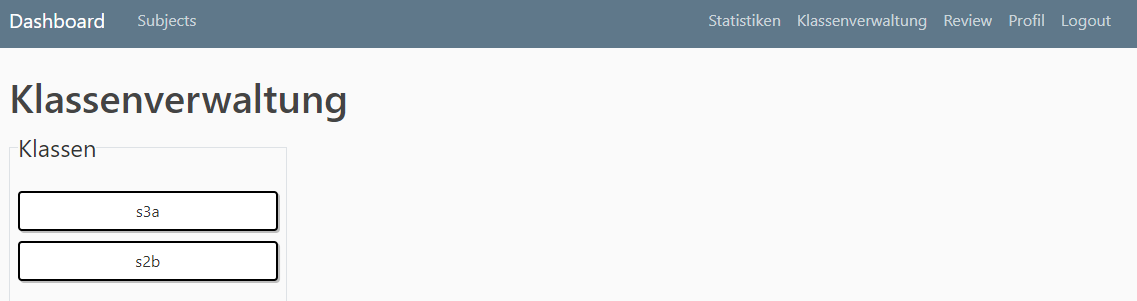
\includegraphics[width=\textwidth, height=\textheight, keepaspectratio]{images/Webseite/Klassenverwaltung_Desktop.png}
		\caption{Anpassung Klassenverwaltung}
	\end{figure}
\end{minipage}	

Nachdem eine Klasse gewählt wurde, werden die klassenspezifischen Informationen geladen und ebenfalls dargestellt. \\

\begin{minipage}{\textwidth}
	\begin{figure}[H]
		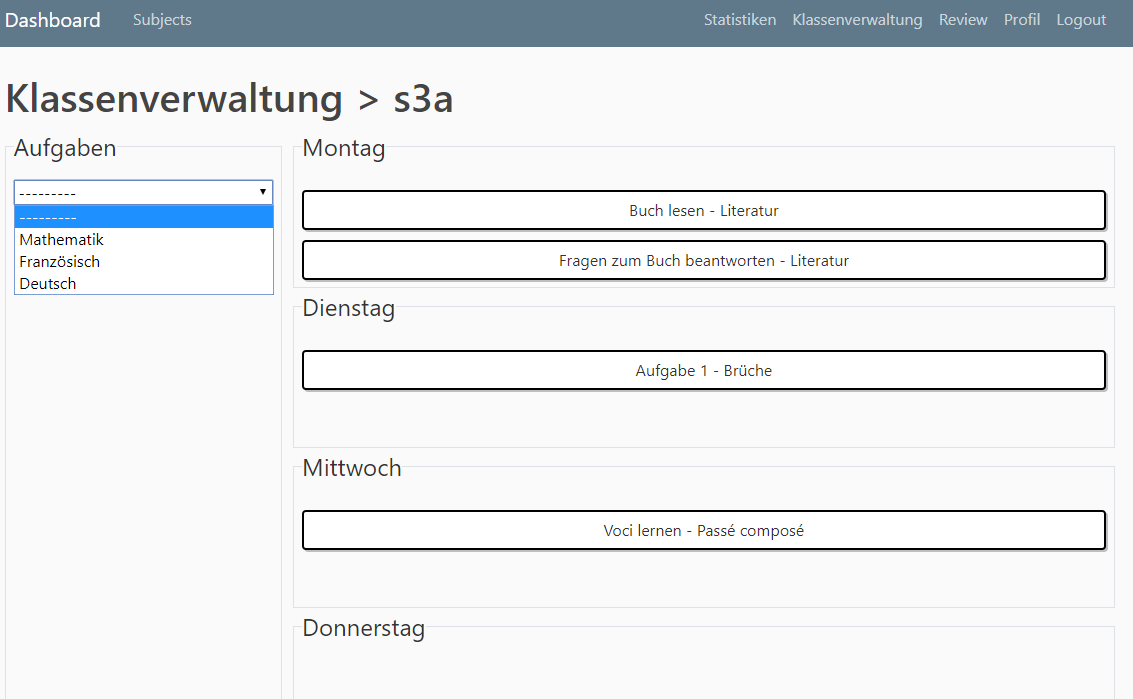
\includegraphics[width=\textwidth, height=\textheight, keepaspectratio]{images/Webseite/Klassenverwaltung_Klasse_Desktop.png}
		\caption{Informationen einer Klasse}
	\end{figure}
\end{minipage}

	\item Die Funktion um eigene Aufgaben mit anderen Lehrpersonen zu teilen wurde entfernt. Standardmässig sind nun alle erstellen Aufgaben für alle Lehrpersonen ersichtlich.
\end{itemize}




%\subsubsection{Funktionale Tests}
%Mit den geschriebenen Tests wurde eine Testcoverage von 97\% erreicht. Bei so hohen Zahlen muss man vorsichtig sein. Nur weil die Testcoverage so hoch ist, heisst es noch lange nicht, dass die Software keine Fehler aufweisst \footcite{test_coverage}. Nur weil eine Zeile Code bei einem Test durchlaufen wird, bedeutet das nicht, dass die Zeile auch getestet wurde. Grundsätzlich gibt es zwei grosse Fehler, die man beim Testen machen kann. Der erste Fehler ist es eine Testcoverage von 100\% anzustreben und sich einZUreden, dass der Code einwandfrei getestet wird. Der zweite Fehler ist es, keinen Wert auf die Testcoverage zu legen. Erreicht man Werte im Bereich von 30\% bis 40\%, ist sofort klar, dass das Testen vernachlässigt wurde. Im allgemeinen gilt, die Qualität der Tests ist ausschlaggebend. Eine hohe Testcoverage erreicht durch sinnvolle Tests ist daher ein anzustrebendes Ziel. 

\subsubsection{Performance Testing}
\label{chapter_performance_tests}
Um sicherzustellen, dass nichtfunktionale Anforderungen wie die Response Time und die Scalability erfüllt werden, wurden Performance Tests durchgeführt. Dafür wurde das Tool Gatling \footcite{performance_tests} verwendet. Um so realitätsgetreu und dementsprechend auch sinnvoll wie möglich zu testen, wurden 300 Schüler, 20 Lehrer und 1 Administrator simuliert, welche die Applikation verwendeten. \\

\textbf{Auswertung:} \\
Insgesamt wurden über einen Zeitraum von 2 Minuten und 15 Sekunden 28'183 Requests abgesetzt. In der Abbildung \ref{request_per_second} ist ersichtlich, wie die Requests über den erwähnten Zeitverlauf verteilt absetzt wurden.

	\begin{figure}[H]
		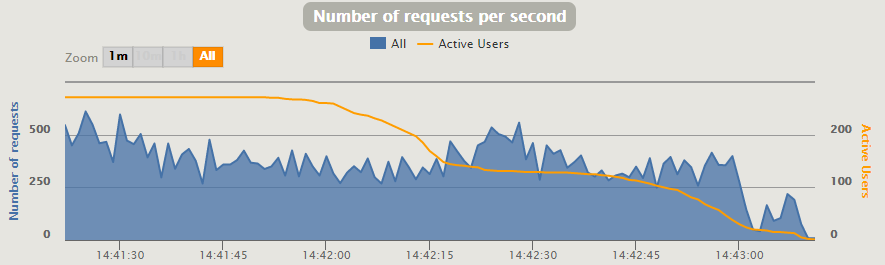
\includegraphics[width=\textwidth, height=\textheight, keepaspectratio]{images/performance_requests_per_second.png}
		\caption{Anfragen pro Sekunde}
			\label{request_per_second}
	\end{figure}

Wie in der Abbildung \ref{performance_tests} ersichtlich ist, benötigte die Applikation bei etwa 6\% der eingegangenen Anfragen etwas länger als eine Sekunde für die Antwort. Grund dafür ist unter anderem das Laden von Bibliotheken, wie zum Beispiel 'jquery-3.1.1.min.js' und 'bootstrap.min.css', welche für die Darstellung der Seite benötigt werden. Diese Bibliotheken wurden zwar statisch in die Applikation eingebunden, was die Performance bereits stark verbesserte, jedoch noch nicht ausreicht. 

	\begin{figure}[H]
		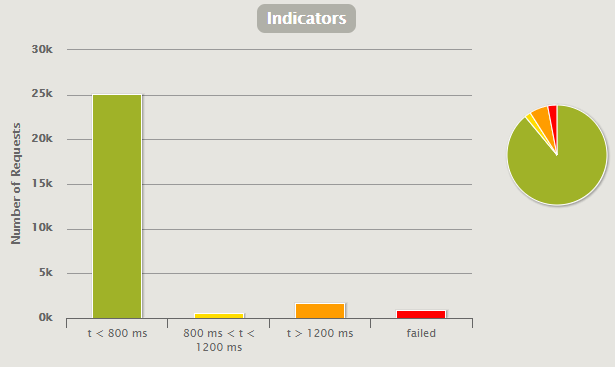
\includegraphics[width=\textwidth, height=\textheight, keepaspectratio]{images/performance_uebersicht.png}
		\caption{Performance Test Übersicht}
			\label{performance_tests}
	\end{figure}


\subsection{Continuous Integration}
\gls{ci} beschreibt das Prinzip, wenn mehrere Entwickler an einem Projekt arbeiten und ihre Änderungen am Code regelmässig in den Master Branch mergen. Dies bietet gleich mehrere Vorteile für die Entwickler. Zum einen werden kleinere Änderungen gemerged. Kleine Änderungen sind einfacher zu handhaben, als wenn grosse Änderungen im Code vorkommen. Bei jedem Merge mit dem master werden die Tests automatisch gestartet. Somit erhalten die Entwickler sehr schnell Feedback, falls Tests fehlgeschlagen sind. Da vorallem kleinere Änderungen gemerged werden, sind die Ursachen der fehlgeschlagenen Tests meist schnell gefunden. Somit lässt sich auch die \gls{mttr} verkürzen.

\subsubsection*{Anbieter}
Bei dieser arbeit wurde Travis als \gls{ci} Anbieter ausgewählt. Bei jeder Änderung am Code auf Github wird Travis mittels Web-Hook benachrichtigt. Der Code wird dann heruntergeladen und gestartet. Die genaue Anweisung, was gestartet und geprüft werden soll, befindet sich im ''.travis.yml'' File. In diesem Fall werden zuerst die drei Docker Container gestartet,  dann wird die Code Qualität geprüft und zum Schluss werden die Tests durchgeführt. Somit sehen die Entwickler schnell, ob die Tests erfolgreich durchgelaufen sind oder nicht. \\

Zusätzlich wurde das Git Repository so konfiguriert, dass ein Pull Request nur in den Master Branch gemerged werden kann, wenn alle Tests erfolgreich durchgelaufen sind und wenn ein Code Review durchgeführt wurde. Somit kann das Risiko vermindert werden, dass nicht lauffähiger Code in den Master gemerged wird. \\

	\begin{figure}[H]
	\begin{center}
			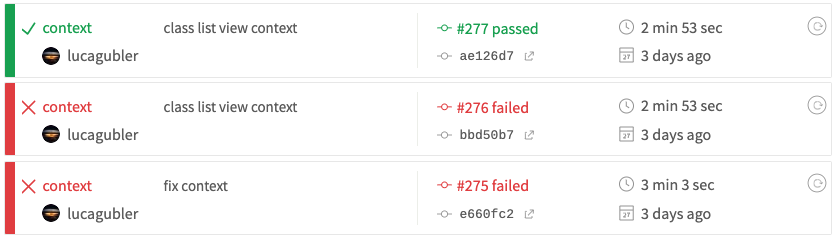
\includegraphics[width=0.8\textwidth, keepaspectratio]{images/travis_build.png}
		\caption{Failed Travis Build}
			\label{fig:trvis_build}
	\end{center}

	\end{figure}

In der Abbildung \ref{fig:trvis_build} kann man ein Beispiel eines fehlgeschlagenen Builds erkennen. Grund dafür war ein fehlende leere Zeile an Ende eines Python Files. Nach dem Einfügen einer leeren Zeile konnte Travis erfolgreich ausgeführt werden. \\

Zu Beginn überlegte man sich, ob man Travis oder Jenkins als \gls{ci} Tool auswählt. Jenkins ist mit über 600 Plugins zwar sehr flexibel und weiter verbreitet als Travis\footcite{travis_jenkins}. Da man aber nur die Basics braucht, ist man nicht auf diese Features angewiesen. Der Hauptgrund, warum man sich für Travis entschied, ist, weil es für öffentliche Git Repositories gratis verwendet werden kann. Jenkins ist zwar auch frei erhältlich, doch man hätte einen eigenen Build Server konfigurieren müssen. 